\chapter{Teori}

\section{Jenis-Jenis Variabel pada \textit{Python}}
Python memiliki 2 jenis variabel yaitu variabel global dan variabel lokal

\subsection{Global}
Variabel global merupakan variabel yang dapat digunakan atau dipanggil oleh semua fungsi. Meskipun variabel tersebut berada di file yang berbeda maupun fungsi yang berbeda.Penddeklarasian variabe global  di tuliskan  pada inisiasi awal file python atau fungi main.

\subsection{Lokal}
Variabel lokal adalah sebuah variabel yang hanya dapat digunakan dan dipanggil dalam satu file saja .

\section{Input dan Output}
Input dimaksud disini adalah bagaimana caranya kita menuliskan kode yang membuat user harus menginputkan sebuah nilai yang mana nilai tersebut akan kita buat outputnya jika tidak di input maka outputnya juga kosong, seperti berikut listing ~\ref{inputoutput}

\lstinputlisting[caption={Input dan Output}, label={inputoutput}, language=Python]{src/inputoutput.py}

dari kode diatas variabel npm akan menyimpan sebuah input yang diisi oleh user, di variabel npm terdapat sebuah fungsi input() yang digunakan untuk  menerima input dari user, dan ada perintah print(npm) berfungsi agar hasil input dari user yang disimpan didalam variabel npm dapat di tampilkan ke layar user.

\section{Contoh Pemakaian Operator Dasar Aritmatika dan Pengubahan Tipe Data}
Untuk pemakaian operator dasar aritmatika dapat dilihat pada listing \ref{aritmatika}

\lstinputlisting[caption={Operator Aritmatika}, label={aritmatika}, language=Python]{src/aritmatika.py}

untuk mengubahan dari tipe data string ke integer dapat menggunakan fungsi int() dan harus dipastikan didalam string tersebut harus berisi integer (angka) tidak boleh string yang lain. Seperti di listing \ref{aritmatika}, saya mencoba memasukkan karakter 1 kedalam variabel bernama string dan tipe datanya string, lalu saya ubah menjadi integer dengan cara int(string) sehingga program mendeteksi bahwa itu adalah integer bukan string dan dapat menjalankan perintah aritmatika tanpa error. Sebalikanya pun sama, dari integer ke dalam string seperti bagian variabel bagi yang isinya integer saya ubah ke string dengan menggunakan fungsi str().

\section{Perulangan}
Untuk perintah perulangan pada python ada 3 yaitu \textbf{for, while, dan nested} penggunaan ketiganya memang berbeda tetapi untuk fungsinya tetap sama yaitu mengulang perintah yang berada di dalam sintaks looping dengan parameter tertentu untuk membuat looping tersebut keluar atau berhenti atau selesai.

\subsection{\textit{for}}
For adalah perulangan yang mana parameter pengulangannya menggunakan list atau range, contoh pada listing \ref{for}

\lstinputlisting[caption={For Loop}, label={for}, language=Python]{src/for.py}

program diatas akan mengeprint sebuah tulisan "Nilai ke-" dari 0 sampai dengan 5.

\subsection{\textit{while}}
While akan mengulang terus menerus jika parameter yang dikembalikan bernilai true dan berakhir jika bernilai false, contoh pada listing \ref{while}

\lstinputlisting[caption={While Loop}, label={while}, language=Python]{src/while.py}

pada kode program diatas akan mengulang terus menerus jika di jawab "ya" dan akan berhenti jika kita jawab "tidak" atau selain "ya".

\subsection{\textit{nested}}
Nested merupakan sebuah pengulangan yang memungkinkan untuk memasukkan parameter pada sebuah pengulangan, contoh pada listing \ref{nested}

\lstinputlisting[caption={Nested Loop}, label={nested}, language=Python]{src/nested.py}

pada kode program diatas kita melihat bahwa looping while yang sebelumnya menggunakan tipe data boolean sekarang bisa menggunakan sebuah parameter khusus yaitu nested sehingga kita bisa menentukan parameter yang diperlukan agar looping while dapat berhenti.

\section{Percabangan}
Percabangan merupakan algoritma yang menentukan sebuah paramater bernilai True atau False.

\lstinputlisting[caption={Percabangan If dan If Bersarang}, label={if}, language=Python]{src/if.py}

program diatas merukapan program yang bisa di bilang bercabang, sehingga hanya bertemu dua jalan True atau False? jika kita lihat pada listing \ref{if} maka pada percabangan pertama kita mengecek sebuah value dari npm apakah kosong atau berisi? jika kosong maka akan mengeprint \textbf{masak lupa sama npm sendiri} jika tidak kosong maka akan print \textbf{npm terisi} dan melanjutkan percabangan yang selanjutkan yaitu mengecek lagi, apakah isi dari npm itu sama dengan \textbf{"11840w6"}? jika sama maka akan mengeprint \textbf{kamu adalah jojo}, jika berbeda maka akan menampilkan pesan \textbf{Apakah kamu hacker?}

\section{Kesalahan yang Sering Terjadi}
Kesalahan yang sering terjadi dalam melakukan semua perintah diatas yaitu biasanya terjadi yaitu:
\begin{enumerate}
\item pertama, biasanya programmer sering salah atau lupa dalam menggunakan operator aritmatika. yaitu ketika memasukan sebuah variabel numerik tidak bisa di ditambah atau dikurang dengan variabel karakter begitu juga sebaliknya.
\item kedua, dalam perulangan biasanya programmer sering lupa dengan menggunakan perintah \textbf{\textit{for i in ...}} pada ... biasanya programmer sering menggunakan angka integer, sehingga program akan error dan tidak bisa melooping sesuai harapan si developer, seharusnya untuk menggunakan looping dengan integer terkhusus untuk for yaitu menggunakan \textbf{\textit{range}}, seperti contoh pada listing \ref{for}
\item ketiga, dalam percabangan biasanya programmer suka salah dalam membandingkan 2 parameter nilai, yang satu variabel string atau karakter, yang satu lagi variabel numerik, sehingga program akan menuju perintah \textbf{\textit{Else}}.
\end{enumerate}

\section{\textit{Try and Except}}
Perintah ini digunakan untuk menangkap sebuah error, dan meneruskan program kita, sehingga program kita ketika terjadi error akan tetap berjalan dan tidak berhenti ditengah jalan. contoh kode bisa dilihat pada listing \ref{tryandexceptlst} dan hasilnya dapat dilihat pada gambar \ref{tryandexceptgbr}

\lstinputlisting[caption={Try and Except}, label={tryandexceptlst}, language=Python]{src/tryandexcept.py}

\begin{figure}[H]
\centering
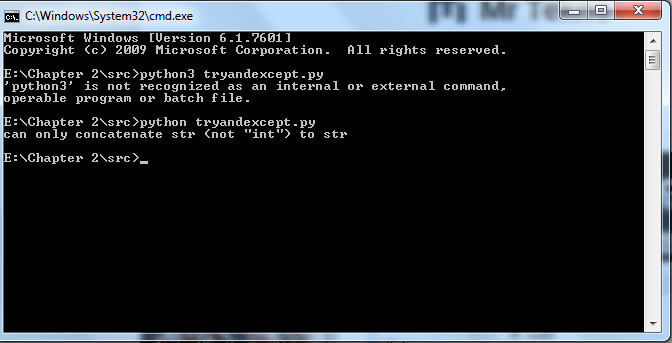
\includegraphics[width=1\textwidth]{figures/tryandexcept.png}
\caption{Gambar Try and Except}
\label{tryandexceptgbr}
\end{figure}

pada program tersebut error menjelaskan bahwa \textbf{"99"} yang merupakan karakter hanya bisa di tambah oleh tipe data yang bertipe karakter juga, tidak bisa dengan integer, begitu juga sebaliknya.